\documentclass[../../../../main.tex]{subfiles}

\begin{document}

\subsection*{第1問}

[解] $r^2 + l = c \quad \cdots \text{①}$

右図から
\[
V = 2 \int_0^r \pi (x^2)^2 \, dx + \pi (r^2)^2 \cdot l
\]
だから①を代入して
\[
V = 2\pi \int_0^r x^4 \, dx + \pi r^4 (c - r^2) \equiv f(r) \quad (0 \le r \le \sqrt{c})
\]
\[
f'(r) = 2\pi r^4 + 4\pi c r^3 - 6\pi r^5 = 2\pi r^3 (-3r^2 + r + 2c)
\]
$c > 0$ より, $-3r^2 + r + 2c = 0$ の 2 実解を $\alpha, \beta$ ($\alpha < \beta$) として, $\beta$ を与える:
\[
\begin{cases}
\cdot f'(0) = 2c > 0 \text{ から } \alpha < 0 < \beta. \\
\cdot \beta = \frac{1 + \sqrt{1+24c}}{6} \le \sqrt{c} \iff 0 \le c(c-1)
\end{cases}
\]

$1^\circ$ $c > 1$ の時

\begin{center}
\begin{array}{c|c|c|c|c|c}
r & 0 & \dots & \beta & \dots & \sqrt{c} \\ \hline
f' & & + & 0 & - & \\ \hline
f & & \nearrow & & \searrow &
\end{array}
\end{center}

$2^\circ$ $0 < c \le 1$ の時

\begin{center}
\begin{array}{c|c|c|c}
r & 0 & \dots & \sqrt{c} \\ \hline
f' & & + & \\ \hline
f & & \nearrow &
\end{array}
\end{center}

従って,
\[
1^\circ \quad c > 1 \text{ の時 } r = \frac{1 + \sqrt{1+24c}}{6}, \quad l = \frac{6c - 1 - \sqrt{1+24c}}{18}
\]
\[
2^\circ \quad 0 < c \le 1 \text{ の時 } r = \sqrt{c}, \quad l = 0
\]

\begin{center}
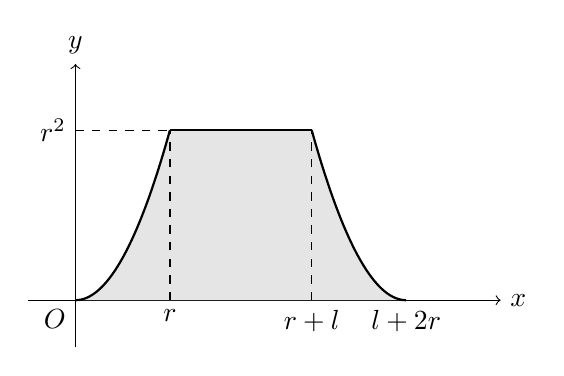
\begin{tikzpicture}[scale=1.2]
  \draw[->] (-0.5,0) -- (4.5,0) node[right] {$x$};
  \draw[->] (0,-0.5) -- (0,2.5) node[above] {$y$};
  \node[below left] at (0,0) {$O$};
  
  \fill[gray!20] plot[domain=0:1,samples=50,smooth] (\x, {1.8*\x*\x}) -- (2.5,1.8) -- plot[domain=2.5:3.5,samples=50,smooth] (\x, {1.8*(1 - (\x-2.5))^2}) -- (0,0) -- cycle;
  
  \draw[domain=0:1,samples=50,smooth,thick] plot (\x, {1.8*\x*\x});
  \draw[thick] (1,1.8) -- (2.5,1.8);
  \draw[domain=2.5:3.5,samples=50,smooth,thick] plot (\x, {1.8*(1 - (\x-2.5))^2});
  
  \draw[dashed] (1,0) -- (1,1.8);
  \draw[dashed] (2.5,0) -- (2.5,1.8);
  \draw[dashed] (0,1.8) -- (1,1.8);
  
  \node[below] at (1,0) {$r$};
  \node[below] at (2.5,0) {$r+l$};
  \node[below] at (3.5,0) {$l+2r$};
  \node[left] at (0,1.8) {$r^2$};
\end{tikzpicture}
\end{center}

\subsection*{第2問}

[解] $t=0$ における P の速度ベクトルが $(2, 0)$ である場合の P のたどりつく領域を, 原点を中心に $60^\circ$ 回転させたものが求める領域である.

P は 1 秒の間に合計距離 2 だけ進む. そこで, $x$ 軸正方向に $\alpha$, $x$ 軸負方向に $\beta$, $y$ 軸正方向に $\gamma$, $y$ 軸負方向に $\delta$ だけ進むとすると ($\alpha \ge 0, \beta \ge 0, \gamma \ge 0, \delta \ge 0$),
\[
\alpha + \beta + \gamma + \delta = 2 \quad \cdots \text{①}
\]
また, たどりつく座標 $(X, Y)$ として
\[
X = \alpha - \beta, \quad Y = \gamma - \delta
\]
である. ①のもとでの $(X, Y)$ の領域を求める. ①から $\delta$ を消去して
\[
X = \alpha - \beta, \quad Y = \alpha + \beta + 2\gamma - 2 \quad (\alpha + \beta + \gamma \le 2, \ \alpha, \beta \ge 0, \ \gamma \ge 0)
\]
より
\[
\begin{pmatrix} X \\ Y \end{pmatrix} = \alpha \begin{pmatrix} 1 \\ 1 \end{pmatrix} + \beta \begin{pmatrix} -1 \\ 1 \end{pmatrix} + \begin{pmatrix} 0 \\ 2\gamma - 2 \end{pmatrix}
\]
$\alpha, \beta$ を固定して $\gamma$ を動かすと, $(X, Y)$ は下図線分上を動く:
\[
0 \le \gamma \le 2 - (\alpha + \beta) \quad (\alpha, \beta \ge 0, \ \alpha + \beta \le 2)
\]
\[
X = \alpha - \beta, \quad -2 + \alpha + \beta \le Y \le 2 - \alpha - \beta \quad \cdots \star
\]

次に $\beta$ を動かす. ($0 < \beta < 2 - \alpha, \ 0 < \alpha < 2$) $\beta = \alpha - X$ を代入して
\[
\begin{cases} -2 + \alpha + (\alpha - X) \le Y \le 2 - \alpha - (\alpha - X) \\ 0 < \alpha - X < 2 - \alpha \end{cases}
\iff \begin{cases} 2\alpha - 2 - X \le Y \le X + 2 - 2\alpha \quad (0 < \alpha < 2) \\ 2\alpha - 2 < X < \alpha \end{cases}
\]
最後に $\alpha$ を動かす. $f(\alpha) = 2\alpha - X - 2$, $g(\alpha) = -2\alpha + X + 2$ とおく.
$0 < \alpha < 2$, $X < \alpha \le \frac{1}{2}(X+2)$ に注意して,
\[
\begin{cases} -2 \le X \le 0 \text{ の時 } f(0) \le Y \le g\left(\frac{1}{2}X + 1\right) \\ 0 \le X \le 2 \text{ の時 } f(X) \le Y \le g\left(\frac{1}{2}X + 1\right) \end{cases}
\]
だから, これを図示して $|X| + |Y| \le 2$ (右上図斜線部) を得る.

これを, 原点を中心に $60^\circ$ 回転させた右上図斜線部が求める領域である (境界含みます).

\begin{center}
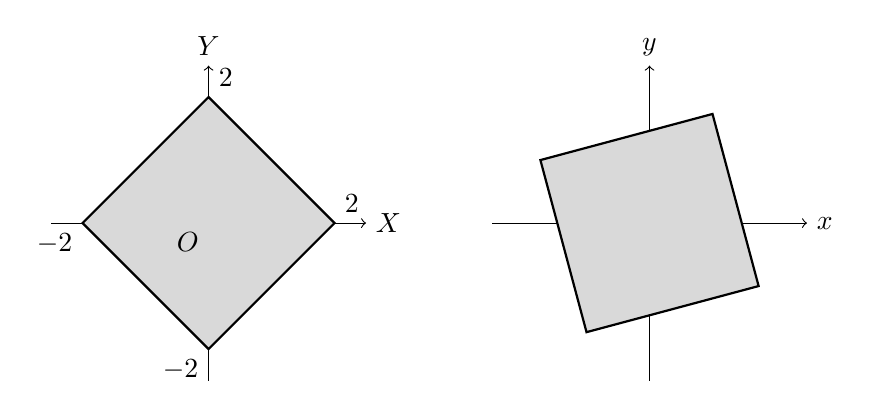
\begin{tikzpicture}[scale=0.8]
  % Diagram 1: |X| + |Y| <= 2
  \begin{scope}[shift={(-3.5,0)}]
    \draw[->] (-2.5,0) -- (2.5,0) node[right] {$X$};
    \draw[->] (0,-2.5) -- (0,2.5) node[above] {$Y$};
    \fill[gray!30] (2,0) -- (0,2) -- (-2,0) -- (0,-2) -- cycle;
    \draw[thick] (2,0) node[above right] {$2$} -- (0,2) node[above right] {$2$} -- (-2,0) node[below left] {$-2$} -- (0,-2) node[below left] {$-2$} -- cycle;
    \node[below left] at (0,0) {$O$};
  \end{scope}
  
  % Diagram 2: Rotated 60 degrees
  \begin{scope}[shift={(3.5,0)}]
    \draw[->] (-2.5,0) -- (2.5,0) node[right] {$x$};
    \draw[->] (0,-2.5) -- (0,2.5) node[above] {$y$};
    \node[below left] at (0,0) {$O$};
    \begin{scope}[rotate=60]
      \fill[gray!30] (2,0) -- (0,2) -- (-2,0) -- (0,-2) -- cycle;
      \draw[thick] (2,0) -- (0,2) -- (-2,0) -- (0,-2) -- cycle;
    \end{scope}
  \end{scope}
\end{tikzpicture}
\end{center}

[別解1 (★以下)]
$\alpha + \beta = k \quad (0 \le k \le 2)$ と固定する.
\[
\begin{cases} X = k - 2\beta \quad (0 \le \beta \le k) \\ -2 + k \le Y \le 2 - k \end{cases}
\]
これを図示すると矩形領域 ($-k \le X \le k, \ -2+k \le Y \le 2-k$) となり, 次に $k$ を動かす. 端点に注目すれば同じ結果が得られる.

[別解2 (★以下)]
条件から $|X| + |Y| \le 2$ だから, 直ちに同図を得る.

\subsection*{第3問}

[解] $P(5 + r\cos\theta, 5 + r\sin\theta)$ ($c = \cos\theta, s = \sin\theta, 0 \le \theta < 2\pi$) とおける.

右図から $Q(13 - r c, -5 - r s)$ であり, $R(-5 - r s, 5 + r c)$ であるから,
\[
\begin{aligned}
\overline{QR}^2 &= (13 - r c + 5 + r s)^2 + (-5 - r s - 5 - r c)^2 \\
&= (18 - r c + r s)^2 + (-10 - r s - r c)^2 \\
&= 18^2 + r^2 + 36 r (s - c) - 2 r^2 s c + 10^2 + r^2 + 20 r (s + c) + 2 r^2 s c \\
&= 18^2 + 10^2 + 2 r^2 + 56 r s - 16 r c \\
&= 18^2 + 10^2 + 2 r^2 + 8 r \sqrt{53} \sin(\theta - \alpha) \quad \left( \text{但し } \tan\alpha = \frac{2}{7} \right)
\end{aligned}
\]
$-\pi \le \theta - \alpha < 2\pi - \alpha$ より, $-1 \le \sin(\theta - \alpha) \le 1$ だから $r > 0$ とあわせて
\[
\begin{cases}
f(r) = \sqrt{18^2 + 10^2 + 2r^2 - 8r\sqrt{53}} = \sqrt{2} |r - 2\sqrt{53}| \\
g(r) = \sqrt{18^2 + 10^2 + 2r^2 + 8r\sqrt{53}} = \sqrt{2} (r + 2\sqrt{53})
\end{cases}
\]
で, $f(r) = 0 \iff r = 2\sqrt{53}$.

\subsection*{第4問}

[解]
(1) $f(x) = \frac{x+t}{x(1-tx)}$,
\[
f'(x) = \frac{t(x^2 + 2tx - 1)}{x^2 (1-tx)^2}
\]
より, 下表を得る:

\begin{center}
\begin{array}{c|c|c|c|c|c}
x & 0 & \dots & -t + \sqrt{t^2+1} & \dots & 1 \\ \hline
f' & & - & 0 & + & \\ \hline
f & & \searrow & & \nearrow &
\end{array}
\end{center}

よって, $\alpha = -t + \sqrt{t^2+1}$ だから $\alpha' = \frac{-1}{\sqrt{t^2+1}} \alpha$.
\[
\frac{d}{dt} f(\alpha) = \frac{(\alpha' + 1) \alpha (1 - t\alpha) - (\alpha + t)(\alpha' - \alpha^2 - 2t\alpha \alpha')}{\alpha^2 (1 - t\alpha)^2}
\]
この分子 $g(\alpha)$ として
\[
\begin{aligned}
g(\alpha) &= \alpha (\alpha' + 1 - t\alpha\alpha' - t\alpha) - (\alpha + t)(\alpha' - \alpha^2 - 2t\alpha\alpha') \\
&= \alpha (\alpha^2 - t\alpha + 1 + t\alpha\alpha') - t\alpha' + t\alpha^2 + 2t^2 \alpha\alpha' \\
&= \alpha^3 + t\alpha^2\alpha' + \alpha - t\alpha' + 2t^2 \alpha\alpha' \\
&= \frac{\alpha}{\sqrt{t^2+1}} \left[ \alpha (1 - 2t\sqrt{t^2+1}) + t + \sqrt{t^2+1} \right] \\
&= 2\alpha \left( t^2 - t\sqrt{t^2+1} + 1 \right)
\end{aligned}
\]
だから下表を得る:

\begin{center}
\begin{array}{c|c|c|c}
t & 0 & \dots & 1 \\ \hline
d\alpha/dt & & - & \\ \hline
df/dt & & + & \\ \hline
(\alpha, f(\alpha)) & (1, 1) & \nwarrow & (\sqrt{2}-1, 3-2\sqrt{2})
\end{array}
\end{center}

よって, グラフは下図:

\begin{center}
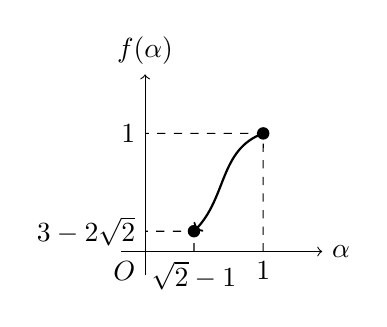
\begin{tikzpicture}[scale=1.5]
  \draw[->] (-0.2,0) -- (1.5,0) node[right] {$\alpha$};
  \draw[->] (0,-0.2) -- (0,1.5) node[above] {$f(\alpha)$};
  \node[below left] at (0,0) {$O$};
  
  \coordinate (A) at (1,1);
  \coordinate (B) at (0.414,0.172);
  
  \draw[dashed] (1,0) node[below] {$1$} -- (A) -- (0,1) node[left] {$1$};
  \draw[dashed] (0.414,0) node[below] {$\sqrt{2}-1$} -- (B) -- (0,0.172) node[left] {$3-2\sqrt{2}$};
  
  \draw[thick,->] (A) to[out=200,in=45] (B);
  \fill (A) circle (1.5pt);
  \fill (B) circle (1.5pt);
\end{tikzpicture}
\end{center}

(2) $-t + \sqrt{t^2+1} \le t \iff \frac{1}{\sqrt{3}} \le t \quad (\because 0 < t < 1 \text{ だから (1) より})$
\[
\beta = \begin{cases} -t + \sqrt{t^2+1} & \left( \frac{1}{\sqrt{3}} \le t \le 1 \right) \quad \cdots \text{①} \\ t & \left( 0 < t \le \frac{1}{\sqrt{3}} \right) \quad \cdots \text{②} \end{cases}
\]
であり, ②の時
\[
f(\beta) = \frac{2\beta}{\beta (1-\beta^2)} = \frac{2}{1-\beta^2} \quad \left( 0 < \beta \le \frac{1}{\sqrt{3}} \right)
\]
は単調増加関数である. これと (1) より, グラフは下図:

\begin{center}
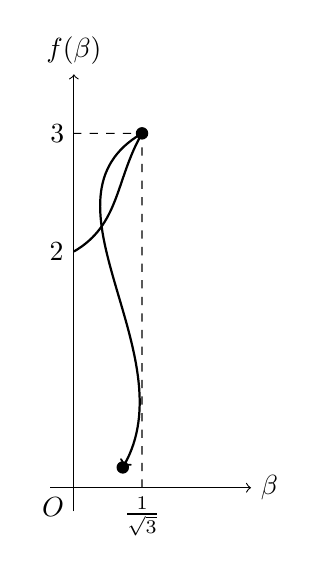
\begin{tikzpicture}[scale=1.5]
  \draw[->] (-0.2,0) -- (1.5,0) node[right] {$\beta$};
  \draw[->] (0,-0.2) -- (0,3.5) node[above] {$f(\beta)$};
  \node[below left] at (0,0) {$O$};
  
  \coordinate (P1) at (0.577, 3);
  \coordinate (P2) at (0.414, 0.172);
  
  \draw[dashed] (0.577,0) node[below] {$\frac{1}{\sqrt{3}}$} -- (P1) -- (0,3) node[left] {$3$};
  
  \draw[thick] (0,2) node[left] {$2$} to[out=30,in=240] (P1);
  \draw[thick,->] (P1) to[out=210,in=60] (P2);
  
  \fill (P1) circle (1.5pt);
  \fill (P2) circle (1.5pt);
\end{tikzpicture}
\end{center}

\end{document}
